\documentclass[11pt,a4paper]{article}
\usepackage[margin=2.5cm]{geometry}
\usepackage{amsmath,amssymb}
\usepackage{booktabs}
\usepackage{enumitem}
\usepackage{xcolor}
\usepackage{tikz}
\usetikzlibrary{arrows.meta,positioning}
\usepackage[colorlinks=true,linkcolor=blue!50!black]{hyperref}

\definecolor{boxbg}{HTML}{EEF3F8}
\definecolor{ink}{HTML}{43505C}
\definecolor{agent}{HTML}{C0392B}
\definecolor{goodF}{HTML}{CFE9D6}
\definecolor{exitF}{HTML}{CFE3F7}
\newcommand{\idea}[1]{\par\smallskip\noindent\colorbox{boxbg}{\parbox{\dimexpr\linewidth-2\fboxsep}{\textbf{Key idea.} #1}}\par\smallskip}

\title{Reading guide\\[2pt]\large The move score head, and why it is built this way}
\author{Companion to \texttt{Chapters/4.Implementation.tex} (the move score)\\and the L3 section of \texttt{fix\_prs\_plan.md}}
\date{}

\begin{document}
\maketitle

\noindent This guide explains one design choice, how the decentralised
policy turns what a robot sees into a choice between its exits. It adds no
new model. The choice is already in the Method chapter as the move score
(\texttt{eq:edgescore}) and is logged as \texttt{[A17]} in
\texttt{thesis-progress/decisions/GAPS.md}. The code change that brings
\texttt{slap-mapd-coupling} into line with it is called L3 (issue \#92).

Part~I is the short version in everyday words. Part~II explains the idea in
more detail. Part~III gives the reasoning, the alternatives that were
weighed, the arguments for the choice and the arguments against it. Nothing here has been measured, and
the places where that matters are listed in the last sections.

\tableofcontents

%================================================================
\part{The short version}

\section{The idea in plain words}

A robot standing at a junction has to pick one of the roads leaving it, or
wait. This guide is about how the policy makes that pick.

\paragraph{How it works today.} The policy gets one description of the robot
and its surroundings. It also has a row of numbered buttons, one for each
road, plus a button for waiting. It must press one button. The buttons are
numbered by the vertex number of the road they lead to, which is only a
label. The description never says which button leads where.

Picture a driver in a country they do not know. At every junction a sign says
``press 1, 2 or 3'' and says nothing about where each button leads. After
many trips the driver may learn that at one particular junction, button 3 is
usually good. But at the next junction button 3 leads somewhere else, so what
was learned is no use there.

\paragraph{The fix.} Look at each road on its own. For every road, ask three
things. Does it get me closer to my target? Is it blocked? Did the robot
standing on it tell me anything? The answers go into one small marking rule,
which gives the road a mark. The same rule marks every road, and the robot
picks among the marks. Waiting gets its own mark.

\paragraph{Why that is better.} The rule ``a road that gets closer and is
free is good'' is true at every junction. So the robot learns it once and
uses it everywhere, whatever the numbers are.

\begin{figure}[h]
  \centering
  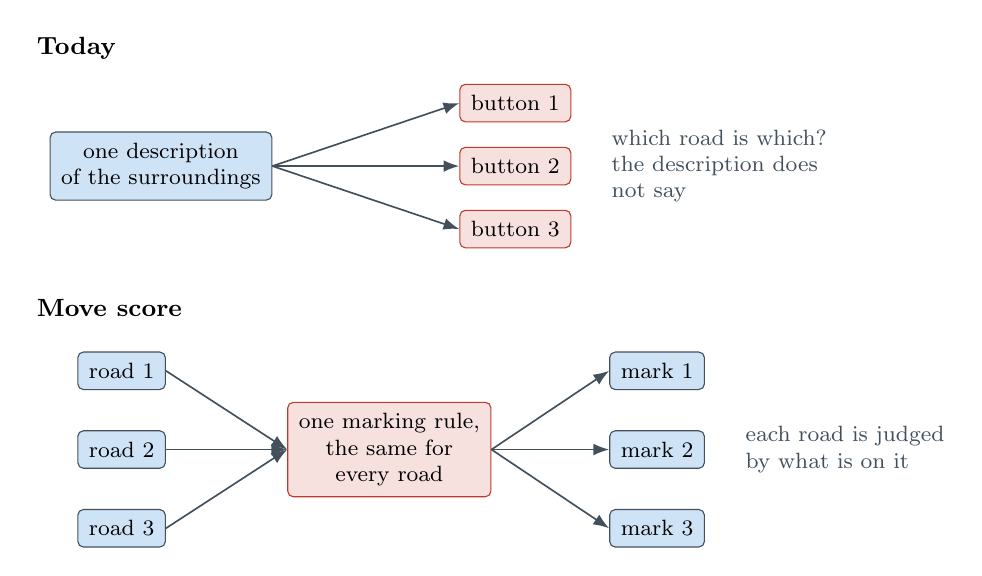
\begin{tikzpicture}[
      box/.style={draw=ink, rounded corners=2pt, fill=exitF, align=center, font=\footnotesize, inner sep=4pt},
      sc/.style={draw=agent, rounded corners=2pt, fill=agent!15, align=center, font=\footnotesize, inner sep=4pt},
      a/.style={-{Latex[length=2mm]}, draw=ink, line width=0.6pt},
      note/.style={font=\footnotesize, text=ink, anchor=west, align=left}]
    % today
    \node[font=\bfseries\small, anchor=west] at (0,2.7) {Today};
    \node[box] (d) at (1.7,1.2) {one description\\of the surroundings};
    \node[sc] (b1) at (6.2,2.0) {button 1};
    \node[sc] (b2) at (6.2,1.2) {button 2};
    \node[sc] (b3) at (6.2,0.4) {button 3};
    \draw[a] (d.east) -- (b1.west);
    \draw[a] (d.east) -- (b2.west);
    \draw[a] (d.east) -- (b3.west);
    \node[note] at (7.3,1.2) {which road is which?\\the description does\\not say};
    % move score
    \node[font=\bfseries\small, anchor=west] at (0,-0.6) {Move score};
    \node[box] (r1) at (1.2,-1.4) {road 1};
    \node[box] (r2) at (1.2,-2.4) {road 2};
    \node[box] (r3) at (1.2,-3.4) {road 3};
    \node[sc] (m) at (4.6,-2.4) {one marking rule,\\the same for\\every road};
    \node[box] (k1) at (8.0,-1.4) {mark 1};
    \node[box] (k2) at (8.0,-2.4) {mark 2};
    \node[box] (k3) at (8.0,-3.4) {mark 3};
    \foreach \i in {1,2,3}{
      \draw[a] (r\i.east) -- (m.west);
      \draw[a] (m.east) -- (k\i.west);
    }
    \node[note] at (9.0,-2.4) {each road is judged\\by what is on it};
  \end{tikzpicture}
  \caption{Today one description feeds numbered buttons. The move score marks each road by looking at it.}
  \label{fig:oldnew}
\end{figure}

\paragraph{What it costs.} The code must remember which road is behind which
button, and which robot stands on which road. The network must also keep what
it already works out about each road, instead of throwing it away. That
bookkeeping is most of the work in L3.

\paragraph{What could go wrong.} A road may lie outside what the robot can
see, and then there is nothing to mark. A robot standing on a road may be too
far away to be heard. Both cases need a rule. Section~\ref{sec:weak} lists
them.

\paragraph{Why not something fancier.} A memory unit such as an LSTM answers
``what happened earlier'', not ``which road is which''. It would also give a
robot information from outside its window, which would spoil the comparison
between the three controllers. Section~\ref{sec:lstm} has the details.

\section{Words used here}

\begin{center}
\small
\begin{tabular}{@{}p{3.2cm}p{11.8cm}@{}}
\toprule
Word & Plain meaning \\
\midrule
exit, road & A way out of the robot's current vertex, that is, a move it may take. \\[2pt]
slot, button & The numbered place for an exit. Slot 0 is wait. Exits are numbered by vertex number. \\[2pt]
summary ($z_i$) & One list of numbers describing the robot and its surroundings. \\[2pt]
embedding & A list of numbers the network builds to describe one vertex. \\[2pt]
message & The embedding another robot reports about its own surroundings. \\[2pt]
score, mark & A number the network gives a move. A higher number makes the move more likely. \\[2pt]
action mask & A rule that removes the moves that do not exist at this vertex. \\
\bottomrule
\end{tabular}
\end{center}

%================================================================
\part{The idea in more detail}

\section{The problem}

A robot's action is a slot number. Slot 0 means wait. Slot $k$ means take
the $k$-th exit of the current vertex, counting the exits by increasing
vertex number. The slot number says nothing about what lies behind the exit.

Figure~\ref{fig:junctions} shows two junctions with three exits each. At
junction A the exits lead to vertices 3, 8 and 12, so they are slots 1, 2
and 3. The target lies beyond vertex 12, so the right move is slot 3. At
junction B the exits lead to vertices 5, 21 and 30, and the target lies
beyond vertex 5, so the right move is slot 1.

A head that must answer slot 3 at one junction and slot 1 at the other,
from nearly the same input, has to tell the junctions apart some other way.

\begin{figure}[h]
  \centering
  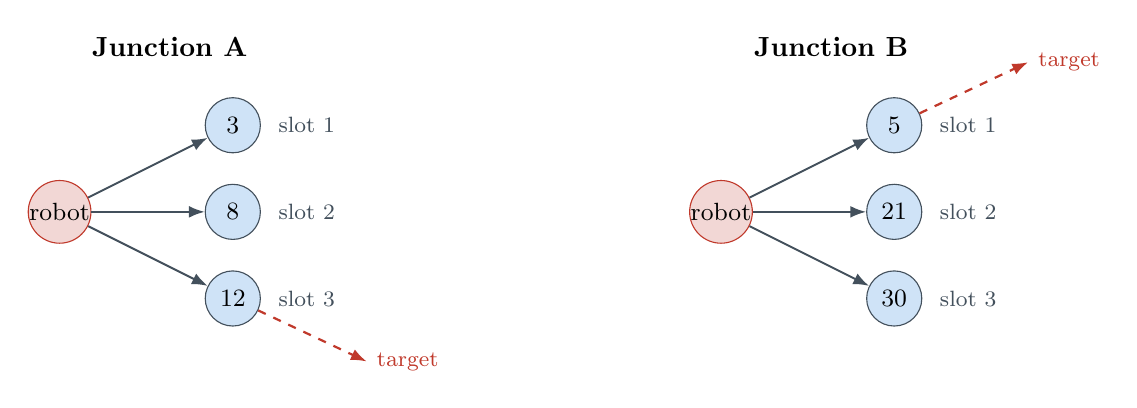
\begin{tikzpicture}[
      v/.style={circle, draw=ink, fill=exitF, minimum size=7mm, inner sep=0pt, font=\small},
      r/.style={circle, draw=agent, fill=agent!20, minimum size=7mm, inner sep=0pt, font=\small},
      e/.style={-{Latex[length=2mm]}, draw=ink, line width=0.7pt},
      t/.style={-{Latex[length=2mm]}, draw=agent, dashed, line width=0.8pt},
      lab/.style={font=\footnotesize, text=ink}]
    % junction A
    \node[font=\bfseries] at (1.4,2.1) {Junction A};
    \node[r] (a0) at (0,0) {robot};
    \node[v] (a1) at (2.2,1.1) {3};
    \node[v] (a2) at (2.2,0) {8};
    \node[v] (a3) at (2.2,-1.1) {12};
    \draw[e] (a0) -- (a1); \draw[e] (a0) -- (a2); \draw[e] (a0) -- (a3);
    \node[lab, right=1mm of a1] {slot 1};
    \node[lab, right=1mm of a2] {slot 2};
    \node[lab, right=1mm of a3] {slot 3};
    \draw[t] (a3) -- (3.9,-1.9) node[right, lab, text=agent] {target};
    % junction B
    \begin{scope}[xshift=8.4cm]
    \node[font=\bfseries] at (1.4,2.1) {Junction B};
    \node[r] (b0) at (0,0) {robot};
    \node[v] (b1) at (2.2,1.1) {5};
    \node[v] (b2) at (2.2,0) {21};
    \node[v] (b3) at (2.2,-1.1) {30};
    \draw[e] (b0) -- (b1); \draw[e] (b0) -- (b2); \draw[e] (b0) -- (b3);
    \node[lab, right=1mm of b1] {slot 1};
    \node[lab, right=1mm of b2] {slot 2};
    \node[lab, right=1mm of b3] {slot 3};
    \draw[t] (b1) -- (3.9,1.9) node[right, lab, text=agent] {target};
    \end{scope}
  \end{tikzpicture}
  \caption{Two junctions. The right slot is 3 at A and 1 at B.}
  \label{fig:junctions}
\end{figure}

\section{What the current head sees}

The current head turns one summary of the robot, $z_i$, into one number per
slot. The summary holds the robot's own embedding, the average of the
messages it received and the crowding $\delta_i(t)$. It holds nothing that
says which exit is which.

Without message passing ($L = 0$) the own embedding is only the features of
the robot's own vertex. The exits do not appear in it at all. With message
passing the exits do appear, but only as an average, because the
message-passing step combines neighbours as an unordered set. An average
cannot say that the closer exit is slot 3.

What the head can learn is a habit tied to the numbering, such as ``at this
kind of vertex, slot 3 is usually good''. That habit does not carry over to
another junction, and it may break when another warehouse is numbered
differently.

\idea{The slot number is bookkeeping. The only thing that says what a move
does is the vertex it leads to, so the head should look at that vertex.}

\section{The fix}
\label{sec:fix}

Score each exit by what is behind it. For one exit, a small network is shown
three things.

\begin{itemize}[leftmargin=1.4em, itemsep=2pt]
  \item The robot's own summary $z_i$.
  \item The embedding of the vertex behind the exit. It says how close that
    vertex is to the target, what role it has and whether it is occupied.
  \item The message of the robot standing on that vertex, or zeros if nobody
    is there.
\end{itemize}

It returns one number. The same network scores every exit at every
junction, so what it learns is ``prefer an exit that gets closer to the
target and is not blocked''. That lesson holds at junction A and at
junction B alike. Waiting gets its own number from $z_i$. The numbers are
placed into the slots in vertex order, and the action mask removes the slots
that do not exist.

Table~\ref{tab:illustration} shows the idea with made-up numbers. At
junction A the robot is 4 away from the target, and at junction B it is also
4 away. One rule picks slot 3 at A and slot 1 at B.

\begin{table}[h]
  \centering
  \small
  \caption{Made-up numbers for the junctions of Figure~\ref{fig:junctions}. Distance is to the target.}
  \label{tab:illustration}
  \begin{tabular}{@{}llrrl@{}}
    \toprule
    Junction & Slot & Vertex & Distance & Occupied \\
    \midrule
    A & 1 & 3  & 5 & no \\
    A & 2 & 8  & 5 & yes \\
    A & 3 & 12 & 3 & no \\
    \midrule
    B & 1 & 5  & 3 & no \\
    B & 2 & 21 & 5 & no \\
    B & 3 & 30 & 6 & yes \\
    \bottomrule
  \end{tabular}
\end{table}

\section{What has to be built}

Three things were missing for this to work.

\begin{center}
\small
\begin{tabular}{@{}p{3.6cm}p{11.4cm}@{}}
\toprule
Piece & Why it is needed \\
\midrule
The embedding behind each exit &
  The encoder already computes it for every vertex in the field of view and
  keeps only the robot's own. The change keeps all of them. \\[3pt]
A slot table &
  The action is a slot number, so the head must know which embedding belongs
  to which slot. The environment records this in the observation, together
  with the robot standing on each exit. \\[3pt]
A rule for exits it cannot score &
  An exit outside the field of view, or a robot that is not among the
  senders heard, leaves the head with no input. The code checks the first
  when the environment is built and gives a zero message for the second. \\
\bottomrule
\end{tabular}
\end{center}

\section{Formally}

For an agent at $v = \ell_i(t)$ and each outgoing neighbour
$w \in N^{+}(v)$, the move score is
\begin{equation}
  \mathrm{logit}(\mathrm{move\ to\ } w) = \mathrm{SCORE}_\theta\bigl(z_i \,\Vert\,
    h_w^{(L)} \,\Vert\, \bar\xi_w(t)\bigr), \qquad
  \mathrm{logit}(\mathrm{wait}) = \mathrm{SCORE}^{\mathrm{wait}}_\theta(z_i),
\end{equation}
where $h_w^{(L)}$ is the final-layer embedding at $w$ and $\bar\xi_w(t)$ is
the message of the agent standing on $w$, zero if there is none. With
communication off, $\bar\xi_w(t)$ is dropped. The policy is the softmax of
these logits plus the action mask $M(v,\cdot)$, as before.

%================================================================
\part{The reasoning}

\section{What the thesis needs from a head}

The thesis compares three learned controllers that differ only in what they
may see. So the head should be a neutral part that is the same for all
three. It should work on warehouses generated from seeds, and it should be
simple enough to finish in the time left. Judged by that, a head that cannot
tell exits apart is the one real defect. Everything else is taste.

\section{The options}

\begin{center}
\small
\begin{tabular}{@{}p{3.4cm}p{4.8cm}p{6.8cm}@{}}
\toprule
Option & What it does & Verdict \\
\midrule
Fixed head as today &
  One output per slot from $z_i$. &
  Cannot tell exits apart. At $L=0$, $z_i$ holds no neighbour information. \\[3pt]
Fixed head plus vertex ID &
  Van Knippenberg's way. &
  The network learns numbers, not geometry. It does not carry over to another numbering. \\[3pt]
Slot concatenation &
  Feed $z_i$ with the embeddings of exits 1 to $d_{\max}$ side by side. &
  Simple, and each exit sees the others. But the weights grow with $d_{\max}$ and each slot learns the same lesson separately. \\[3pt]
Sort exits by distance to the target &
  Slot 1 is always the exit closest to the target. &
  A fixed head then works. But it builds the shortest-path planner into the policy and contradicts \texttt{[A15]}. \\[3pt]
Score every vertex in view &
  The action is ``which vertex''. &
  No slot table, but the action space is no longer small and shared, and it contradicts \texttt{[A15]}. \\[3pt]
Dot-product attention &
  Score is a dot product, not a network. &
  Fewer weights, but it learns fewer interactions. The thesis says ``one small fully connected network'', and attention is future work (\texttt{[A18]}). \\[3pt]
\textbf{Per-edge head} &
  One shared network scores each exit. &
  Same lesson at every junction, any number of exits, weights independent of $d_{\max}$. \\
\bottomrule
\end{tabular}
\end{center}

\section{Why not an LSTM}
\label{sec:lstm}

An LSTM does not make the head cheaper and does not fix the problem. There
are three ways to use one.

\paragraph{As memory across timesteps.} This gives the robot a hidden
state. It answers a different question, ``what happened earlier'', and does
not say which exit is which, because that is a spatial question at a single
timestep. It also works against the thesis. The three controllers differ
only in their window (\texttt{tab:information}), and the critic reads the
same window as its policy (\texttt{[A13]}). A hidden state carries
information from outside that window, so a difference between the
controllers could come from memory and not from the window.

It is also costly to build. The state would have to be carried through
episodes by RLlib. The learned message recomputes each sender's embedding
with the current weights, so each sender's state would need recomputing as
well.

\paragraph{As a sequence over the exits.} Pointer networks were first
written with an LSTM. But an LSTM reads the exits in order, so the result
depends on the numbering again, which is what the move score removes. It
also costs more than a small network per exit, because it has four gates and
runs one step after another.

\paragraph{Inside the message passing.} A recurrent unit in place of
$\psi_r$ is a known design. It changes the encoder and not the head, and it
adds weights.

\section{Van Knippenberg and PRIMAL}

Read in the paper (\texttt{knippenberg21a.pdf}). The action space is ``a
small action space \dots\ shared among all agents, and across problem
instances'', defined as local movement options, one move across each
outgoing edge plus wait. The model is a graph convolution, then fully
connected layers with ReLU, then a softmax over one fixed output vector.
Every node carries a node ID. That ID is the only thing in the input that
could tell two outgoing edges apart, and the paper does not say how move $k$
is matched to an edge. An invalid move is treated as a penalised wait.

PRIMAL (\texttt{1809.03531v3.pdf}) ends its network in an LSTM, on lattice
graphs only. Van Knippenberg dropped the LSTM, and the thesis has none.

The move score keeps van Knippenberg's principle. The action set is the same
small shared set, $d_{\max}+1$ slots, and the head is, if anything, more
shared than theirs. What changes is how the logits are computed. The thesis
already says so in its action-space paragraph, ``this is where the head
departs from van Knippenberg''. An earlier decision (\texttt{[A16]}) kept
their head and noted the node-ID caveat. \texttt{[A17]} replaced it.

\section{Arguments for the per-edge head}

\begin{enumerate}[leftmargin=1.6em, itemsep=3pt]
  \item \textbf{It removes a real defect.} The current head cannot tell
    exits apart, and the reason is visible in what $z_i$ holds.
  \item \textbf{One lesson, learned once.} The shared network learns ``prefer
    an exit that gets closer and is free'' from every junction the robots
    visit, and not once per slot.
  \item \textbf{Numbering does not matter.} Relabelling the slots only
    permutes the logits. This is a direct test of the thesis claim that the
    vertex numbering no longer affects what the policy learns.
  \item \textbf{It is neutral between the controllers.} The centralised and
    section-based controllers read all their robots' vertices from one
    shared pass, so the same head fits them. No controller gets a special
    head, which keeps the window comparison clean.
  \item \textbf{A message sits at the exit it concerns.} The message of the
    robot on an exit is an input to that exit's score. This is what lets
    communication help the choice of a move, and it is the reason
    \texttt{[A17]} gave.
  \item \textbf{Any number of exits.} The weights do not depend on $d_{\max}$.
  \item \textbf{Small cost.} The head runs a few small networks per robot.
    The encoder is the expensive part, and the learned message already
    multiplied it by one plus the number of senders. This is from counting
    operations. It has not been profiled.
  \item \textbf{Little RLlib machinery.} The change is what the actor
    network reads. It needs no connector, unlike the message option that was
    rejected in L2b.
  \item \textbf{The thesis already commits to it.} The code catches up with
    the text, and not the other way round.
\end{enumerate}

\section{Arguments against, and weak points}
\label{sec:weak}

\begin{enumerate}[leftmargin=1.6em, itemsep=3pt]
  \item \textbf{Each exit is scored alone.} The head cannot say ``both exits
    are blocked, so wait'' except through the softmax and $z_i$. Slot
    concatenation could model that directly.
  \item \textbf{The plumbing has a risk.} RLlib has to pass a head more than
    one tensor. In the RLlib source the training forward pass hands the
    actor's embedding straight to the policy head, so a dictionary should
    work. The inference and value paths were not checked in the source. The
    build starts with a spike for this, and falls back to one flat tensor if
    it fails.
  \item \textbf{Exits can lie outside the field of view.} The field of view
    uses cost distance, the depth $d_{\mathrm{obs}}$ is an integer, and the
    generator can draw random edge costs between 0.5 and 2.0. Depth 1
    appears in five places in the tests and examples. The code will check at
    construction that every exit is inside the view, and this may reject
    some existing configurations. It has not been run.
  \item \textbf{An unheard sender gives a zero message.} The number of
    messages is capped, and most test and example configurations use 1 or 2.
    A junction with three occupied exits can then have an exit without a
    message. The thesis says ``if there is one'' and does not cover the cap.
  \item \textbf{It adds a choice to the padding-caps decision.} The view must
    keep every exit, and two checks follow from that. This touches the open
    decision on padding caps (decision 15).
  \item \textbf{Nothing was measured.} The claim that the fixed head cannot
    learn the lesson rests on what $z_i$ holds, not on a run.
  \item \textbf{Numbering may carry direction.} If the generator numbers
    vertices systematically, slots may behave like directions, and the fixed
    head could be good enough on that family. I have not tested this.
  \item \textbf{Compute is not an argument.} The head is cheap either way, so
    a cheaper head would save almost nothing. A simpler head saves
    engineering effort, and slot concatenation needs nearly the same
    changes.
\end{enumerate}

\idea{If the thesis wants evidence for the choice, run the current fixed head
on one small instance before L3 lands and keep the number. Then a reviewer's
question ``why per-edge?'' has a measured answer. This depends on the
training budget (decision 2).}

\section{Decision 14, the extra trunk}

Today a shared hidden layer, the trunk, sits between $z_i$ and both the
policy and the value output. With the move score the policy no longer reads
a trunk, it reads the three inputs of Section~\ref{sec:fix}. A trunk shared with the
value would then serve only the value and the wait score.

The author decided on 2026-10-13 to drop it (option a), so the move score,
the wait score and the value are three small networks that each read their
own input. This matches the thesis, where the value head is ``a fully
connected network with ReLU activations over $z_i$''. It also closes the gap
item ``the head adds its own trunk'' by making the code match the text.

The text needs no edit, but the figure does. \texttt{fig:architecture} draws
one ``fully connected + ReLU'' box between the readout and both heads, which
is the trunk. Under (a) that box goes and the readout feeds the three
networks. The figure edit is still to be made.

\section{What is not verified}

\begin{itemize}[leftmargin=1.4em, itemsep=2pt]
  \item No part of this has been trained or timed. The claims about what the
    fixed head can learn come from reading the code.
  \item The RLlib inference path for a head with several inputs.
  \item Whether existing test and example configurations pass the new
    field-of-view check.
  \item How often the zero message for an unheard sender occurs.
\end{itemize}

\section{What the change does}

The code change, L3, is built on its own branch and is run and pushed by the
author. It makes three changes, in this order.

\begin{enumerate}[leftmargin=1.6em, itemsep=2pt]
  \item The observation gets a slot table, and the field of view always keeps
    every exit.
  \item The encoder hands over the embedding of every vertex, not only the
    robot's own.
  \item The head becomes the move score, the wait score and the value, and the
    RLlib module is wired to it.
\end{enumerate}

The full list of files, tests and open choices is in the L3 section of
\texttt{fix\_prs\_plan.md}.

\end{document}
